\documentclass[runningheads,a4paper]{llncs}

\usepackage{amssymb}
\setcounter{tocdepth}{3}

\usepackage{graphicx}
\usepackage{subcaption}
\usepackage{caption}
\usepackage{url}

\urldef{\mailsa}\path|alexa.schlegel@gmail.com|
\newcommand{\keywords}[1]{\par\addvspace\baselineskip
\noindent\keywordname\enspace\ignorespaces#1}

\renewcommand*\familydefault{\sfdefault}

\begin{document}

\mainmatter  % start of an individual contribution

% first the title is needed
\title{Temporal Development of Overlapping Communities in Co-Authorship Networks}

% a short form should be given in case it is too long for the running head
\titlerunning{Temporal Development of Overlapping Communities}

% the name(s) of the author(s) follow(s) next
%
% NB: Chinese authors should write their first names(s) in front of
% their surnames. This ensures that the names appear correctly in
% the running heads and the author index.
%
\author{Alexa Schlegel%
}
%
\authorrunning{Temporal Development of Overlapping Communities}
% (feature abused for this document to repeat the title also on left hand pages)

% the affiliations are given next; don't give your e-mail address
% unless you accept that it will be published
\institute{Freie Universit{\"a}t Berlin, Institute of Computer Science\\
\mailsa\\
}

%
% NB: a more complex sample for affiliations and the mapping to the
% corresponding authors can be found in the file "llncs.dem"
% (search for the string "\mainmatter" where a contribution starts).
% "llncs.dem" accompanies the document class "llncs.cls".
%

\toctitle{Temporal Development of Overlapping Communities in Co-Authorship Networks}
\maketitle


\begin{abstract}
Detection of overlapping communities plays an important role when it comes to analyzing scientific collaboration using social networks. This paper focuses on describing a method to analyze the temporal development of overlapping communities within co-authorship networks. The paper mainly relies on the work of Palla~et~al. using the clique percolation method for community extraction. The main goal was to find and understand an appropriate algorithm, which can be applied to an existing dataset of scientific publications. Implications regarding further actions and time complexity are discussed.

\keywords{co-authorship networks, scientific collaboration networks, overlapping community detection, temporal analysis, clique percolation, dynamic communities}
\end{abstract}

\section{Introduction and Motivation}
A \emph{social network} is a representation of a social structure consisting of actors, e.g.~individuals, affiliations, and their social interactions.
The network model conceptualizes e.g.~social, economic or political structures as lasting patterns of interactions between actors.~\cite{wasserman1994social}

A \emph{co-authorship network} is a scientific collaboration network, where actors are scientists and the social interaction is collaboration work resulting in publishing papers together.
In mathematical terms networks are graphs, therefore they consist of nodes (vertex) and links (edges).
In a co-authorship network nodes are individual authors who are considered connected if they co-authored a paper.~\cite{newman2001structure}

Usually, those networks are used to study patterns of scientific collaboration in different fields, their development over time, identify key people regarding different network measurements, detection and evolution of communities and many more. See~\cite{barabasi2002evolution}, \cite{newman2001structure} and \cite{newman2004coauthorship} for more details.

This seminar paper is motivated by a dataset consisting of $2.277$ publications related to geochemistry focusing on papers talking about stable metal isotopes (e.g.~potassium, magnesium, lithium, silicon). This data was used to build a cummulated co-authorship network using an very simple approach to model collaboration.

The dataset was collected using the bibliographic database scopus\footnote{\url{http://www.scopus.com/}} and includes publications starting from 1997/98 until 2014.
The dataset consists of authors, co-authors, title, year, abstract and affiliations.
A basic network analysis had already been conducted for example centrality measurement, community detection, degree distribution and average degree.

As the data set includes temporal information~(publishing year), the following question arises: How do communities within this type of co-authorship network evolve over time? In geochemistry people often tend to focus on one isotope system, and stick to this topic for a long time. Do researchers in geochemistry really focus on one specific topic or do they change the field over time?

The goal of this seminar paper therefor is to find and explain an already established and well-understood method for analyzing the temporal development of communities within co-authorship networks. The main point is to understand the underlying algorithm in detail and to find out implications and challenges when applying this method to the geochemistry dataset.

\section{Related Work}
\label{related}
The related work focuses on algorithms for community detection especially for co-authorship networks and how to track those detected communities over time.
``Most real world networks contain parts in which nodes are more highly connected to each other than to the rest of the network, those sets are usually called clusters, communities, cohesive groups or modules, they have no widely accepted, unique definition.''~\cite{palla2005uncovering}
The way ``more highly connected'' is precisely defined makes the difference between community detection algorithms.
It depends on the heuristic which is employed to identify communities.~\cite{porter2009communities}

Fortunato~\cite{fortunato2010community} gives an extended overview about various types of community detection algorithms.
To explain any, would exceed the scope of this work.
For example, traditional methods include algorithms based on graph partitioning, hierarchical clustering and spectral clustering.
There are also divisive and agglomerative algorithms.
The best-known one from this category is Girvan and Newman~\cite{girvan2002community}.

Most algorithms determine distinctive sets of communities, so a node can only belong to a single community. Most real world networks consist of overlapping and nested communities e.g.~friendship network of a person~\cite{palla2005uncovering}.
Fortunato~\cite{fortunato2010community} gives also an overview about algorithms detecting overlapping communities.
The best known and widely cited is the \emph{clique percolation method (CPM)} by Palla et~al.~\cite{palla2005uncovering}.
There is an implementation provided by the authors, called \emph{CFinder}\footnote{CFinder is a tool which implements the clique percolation method by Palla and finding and visualizing overlapping dense groups of nodes in networks. \url{http://www.cfinder.org/}, 05.12.2015, 22:43}, and an implementation in the R igraph library\footnote{\url{http://igraph.wikidot.com/community-detection-in-r#toc0}, 05.12.2015, 22:45}.

Not only overlapping communities exists in networks, also communities are structured in an hierarchical way.
Recent work on algorithms detecting hirachical and overlapping sturctures  include~\cite{1367-2630-11-3-033015}, \cite{Cui201485} and~ \cite{Shen20091706}.

Looking at the temporal development of communities ``the main phenomena occurring in the lifetime of a community are: birth, growth, contraction, merger with other communities, split, death''~\cite{fortunato2010community} (see figure~\ref{fig:evolution}).
The detection of dynamic communities has been studied by Palla et~al.~\cite{palla2007quantifying} using CPM for each snapshot of the graph. Further information on dynamic communities can be found in section 13 of~\cite{fortunato2010community}.

\begin{figure}
	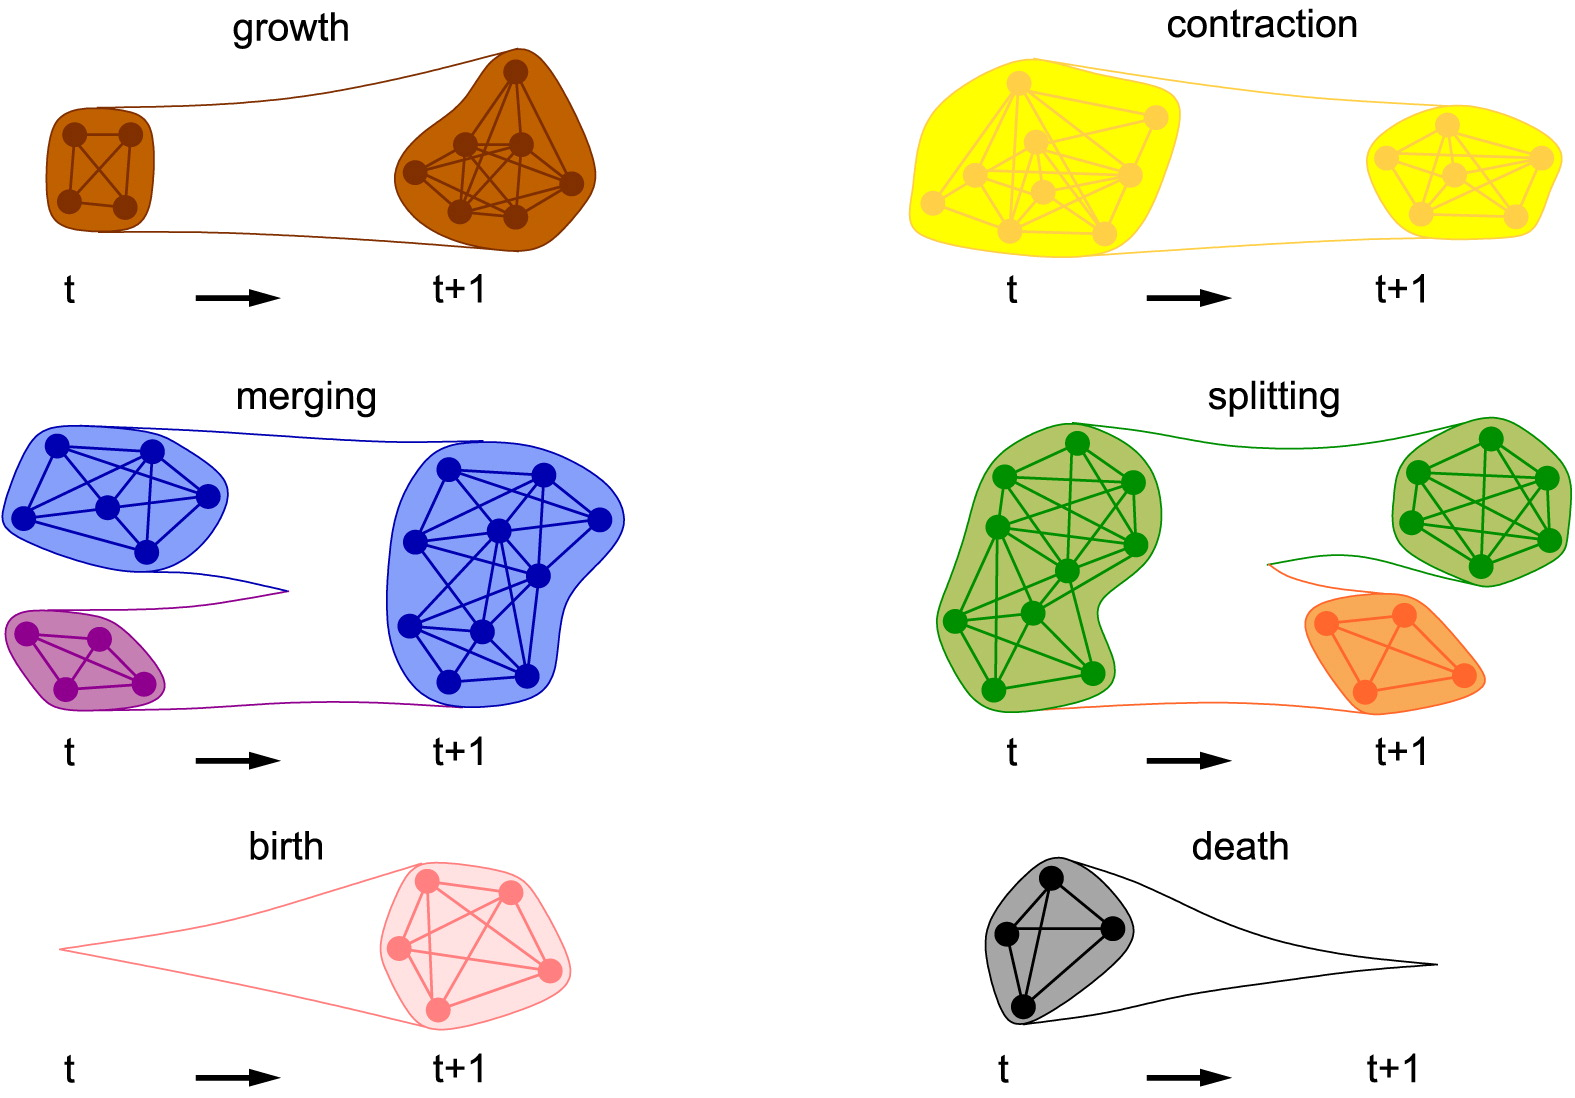
\includegraphics[width=\textwidth]{villsize.jpg}
	\caption{lifetime of a community}
	\label{fig:evolution}
\end{figure}

As CPM is a widely used method for detecting overlapping communities I will explain this method in more detail. The following sections describe the CPM and also the temporal algorithm mainly based on the two papers of Palla et~al.~\cite{palla2005uncovering} and~\cite{palla2007quantifying}.

\section{Clique Percolation Method}
\label{cpm}
The clique percolation method (CPM) developed by Palla et~al.~\cite{palla2007quantifying} is used to identify overlapping communities in unweighted and undirected networks.
The authors tested and evaluated their method using a co-authorship network, protein-protein interaction network, word associations network and a network constructed from variables within the source code of an open source FTP program.
The following section explains the algorithm and summarizes the main findings of the paper regarding co-authorship networks.

The underlying community definition relies on the fact that a community consists of fully connected subgraphs, called \emph{cliques}.
\emph{$k$-cliques} are fully connected subgraphs with $k$ nodes.
In figure~\ref{fig:cliques} an example of $\{3,4\}$-cliques are given.
A community, in this context, is called a \emph{$k$-clique-community}, which is defined as a union of all $k$-cliques, which can be reached from each other through a number of \emph{adjacent $k$-cliques}.
Two $k$-cliques are called adjacent if they share $k-1$ nodes.
In figure~\ref{fig:rolling} the so called $k$-clique template rolling is visualized for a $3$-clique.
A $k$-clique-community is best described by relocating one node until all nodes of the community are discovered.

\begin{figure}
    \centering
    \begin{subfigure}[b]{0.3\textwidth}
        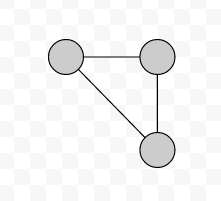
\includegraphics[width=\textwidth]{3-clique}
        \caption{3-cliquel}
        \label{fig:3clique}
    \end{subfigure}
    ~ %add desired spacing between images, e. g. ~, \quad, \qquad, \hfill etc. 
      %(or a blank line to force the subfigure onto a new line)
    \begin{subfigure}[b]{0.3\textwidth}
        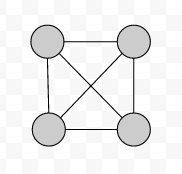
\includegraphics[width=\textwidth]{4-clique}
        \caption{4-clique}
        \label{fig:4clique}
    \end{subfigure}
    ~ %add desired spacing between images, e. g. ~, \quad, \qquad, \hfill etc. 
    %(or a blank line to force the subfigure onto a new line)
    \begin{subfigure}[b]{0.3\textwidth}
        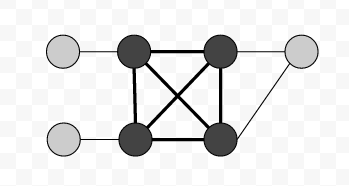
\includegraphics[width=\textwidth]{cliqueinside}
        \caption{4-clique inside a graph}
        \label{fig:cliqueInside}
    \end{subfigure}
    \caption{Examle of cliques}\label{fig:cliques}
\end{figure}

\begin{figure}
	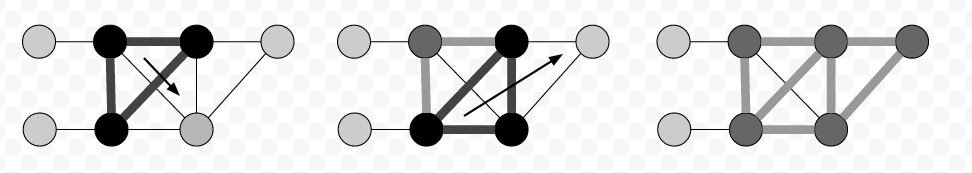
\includegraphics[width=\textwidth]{rolling.png}
	\caption{Template rolling for a $3$-clique}
	\label{fig:rolling}
\end{figure}

\subsection{Algorithm}
\label{cpm-algo}
The starting point for the algorithm is an undirected and unweighted graph. In section \ref{cpm-construction} we talk about generating the  unweighted co-authorship graph.
Based on the explained community definition the algorithm consists of the following steps:

\begin{enumerate}
\small
\item[(1)] Find all maximal cliques.
\item[(2)] Prepare clique-clique overlap matrix, or clique graph.
\item[(3)] Threshold the matrix with a certain $k$.
\item[(4)] Each connected component in the clique graph form a $k$-clique-community.
\item[(5)] Post-processing.
\end{enumerate}

\subsubsection{(1) Find all maximal cliques}
Instead of finding all $k$-cliques, as a first step, the algorithm searches for all maximal cliques. Instead of finding all $k$-cliques, which is a polynomial problem, his can be done in exponential time the authors state.
Maximal cliques cannot be subsets of larger cliques.
That is why they are detected in decreasing order of their size.
The largest possible clique size $s_{max}$ is determinde by the maximal degree $d_{max}$ found in the network.

\begin{enumerate}
\small
\item[(1)] Determine $s=s_{max}$.
\item[(2)] Repeatedly choose a node $v$ from the graph:
	\begin{enumerate}
		\item[(2.1)] Extract all cliques of size $s$ containing $v$.
		\item[(2.2)] Delete the node and its edges.
	\end{enumerate}
\item[(3)] When no nodes are left set $s=s-1$ and start with (2) on the original graph.
\end{enumerate}

The set of already found cliques do influence the found cliques in later steps, as the later found cliques are smaller.
The detailed algorithm for step (2.1) finding cliques of size $s$ of $v$ can be looked up in supplementary material to the paper on section 1.1.2, page 3.
The result of this step is a set with size $n_c$ of all maximal cliques, an example can be seen in figure~\ref{fig:3clique}.

\begin{figure}
\begin{center}
	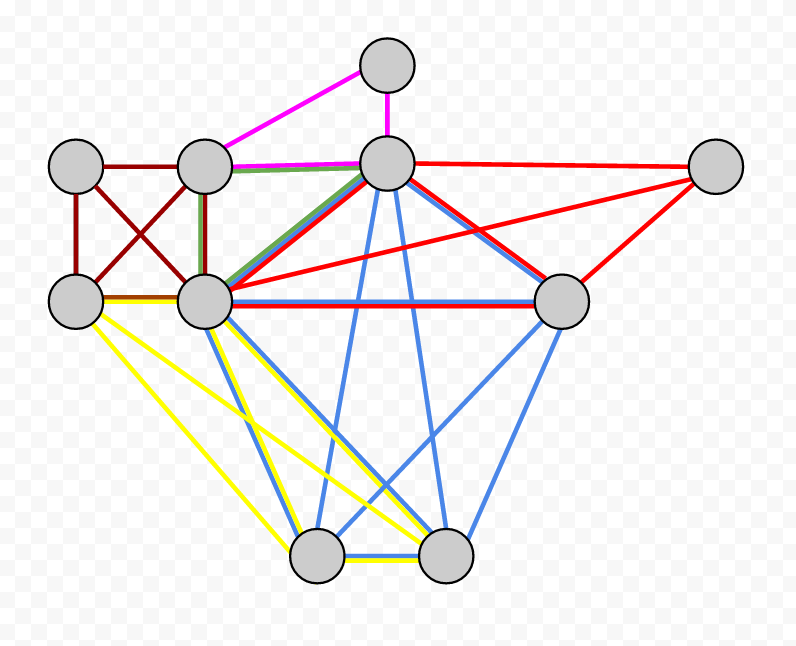
\includegraphics[width=0.8\textwidth]{allmaxcliques.png}
		\caption{All maximal cliques in a graph. Each color represents a maximal clique.}
		\label{fig:allmaxcliques}
\end{center}
\end{figure}

\subsubsection{(2) Prepare clique-clique overlap matrix, or clique graph}
The dimension of the overlap matrix is $n_c \times n_c$. Each row and column represent a clique.
All non-diagonal matrix elements represent the number of nodes those cliques share.
The diagonal entries represent the size of the corresponding clique.
This matrix is only generated once.
In figure~\ref{fig:matrix} the clique-clique overlap matrix of the graph of figure~\ref{fig:allmaxcliques} and the coressponding clique graph is shown.

\begin{figure}
\begin{center}
	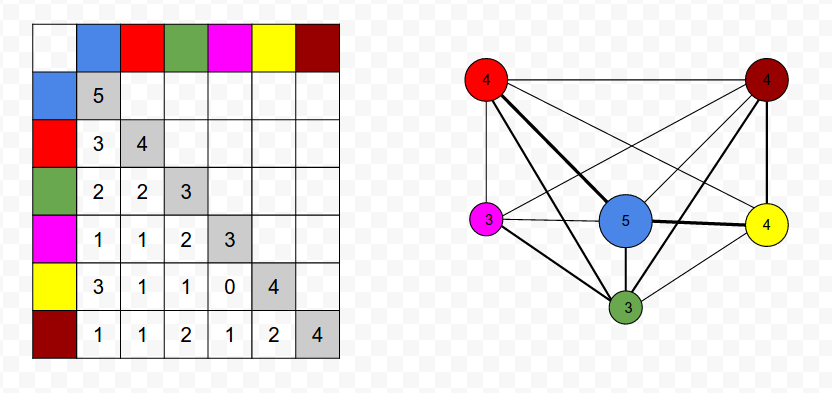
\includegraphics[width=0.8\textwidth]{matrix.png}
		\caption{The clique-clique overlap matrix and the corresponding clique graph. The number inside the node is the number of nodes belonging to that community, the width of the edge represents the shared nodes.}
		\label{fig:matrix}
\end{center}		
\end{figure}


\subsubsection{(3) Threshold the matrix}
All off-diagonal entries smaller than $k-1$ and diagonal entries smaller than $k$ are set to $0$.
The remaining elements are set to $1$, resulting in a binary matrix, representing a network of cliques. The thresholding can be done repeatedly without calculating a new matrix, see figure~\ref{fig:matrixtrashed}.

\begin{figure}
\begin{center}
	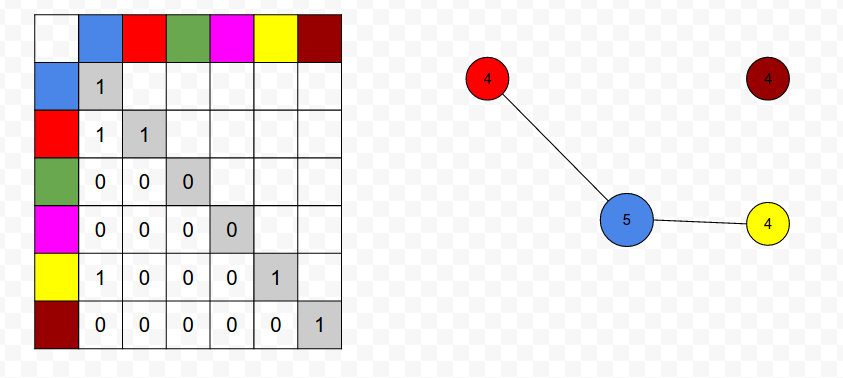
\includegraphics[width=0.8\textwidth]{matrixtrashed}
		\caption{This is the resulting clique graph after the thresholding with $k=4$. All connected components do represent a $k$-clique-community. In this example are two communities.}
		\label{fig:matrixtrashed}
\end{center}
\end{figure}
 
\subsubsection{(4) Each connected component in the clique graph form a $k$-clique-community.}
In the resulting graph we need to look for connected components, those represent the $k$-clique-communities, see figure~\ref{fig:result}.

\subsubsection{(5) Post-processing.}
The last step of the algorithm assigns left over nodes, if possible, to communities. A node which is only connected to one certain community and is not part of a community already is associated with this community. The number of nodes belonging to a community can be increased.

\begin{figure}
\begin{center}
	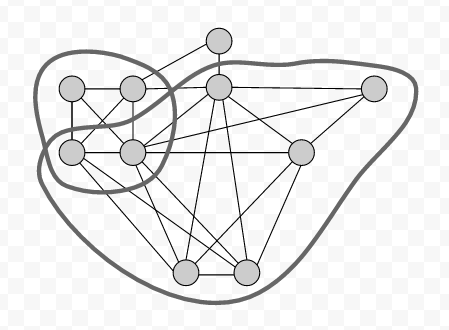
\includegraphics[width=0.8\textwidth]{result}
		\caption{Here the two resulting $k$-clique-communities are shown.}
		\label{fig:result}
\end{center}
\end{figure}


\subsection{Construction of the co-authorship network}
\label{cpm-construction}
The edge weights are calculated with $$\frac{n}{n-1}$$ with $n$ beeing the number of authors per publication.
This results in modeling the collaboration between fewer authors as more intensive than the collaboration between a higher number of authors.  
To generate an unweighted network all edges with an edge weight below a certain threshold $w^*$ need to be removed, all others edge weight are replaced by weight $1$. Increasing $w^*$ results in fewer edges throughout the network, but stronger links and fewer detected communities.

In addition, a good $k$ needs to be chosen. When $k$ is increased the detected $k$-clique-communities shrink, but at the same time become more cohesive (stronger connected).
So a good balance between $k$ and $w^*$ needs to be found resulting in a community structure which is highly structured.

The authors state that $k$ is usually between $3$ and $6$.
If the number of links in a network is increased above some point a giant component evolves and covers the underlying community structure.
So for each $k$ the threshold $w^*$ is lowered until the largest component becomes twice as big as the second largest component. For really choosing the best $k$ some further characteristics describing the community structure need to be investigated, see Supplementary Information of~\cite{palla2005uncovering} for more details.

\subsection{Main Findings of the paper}
Overlaps in networks are significant. The distributions introduced in the paper (community size, community degree, overlap size, membership number) reveal universal features of networks. The network of communities has non-trivial correlations and specific scaling properties.~\cite{palla2005uncovering}

\section{Community Evolution}
\label{evolution}
Palla et~al.~\cite{palla2007quantifying} developed an algorithm based on clique percolation (see section~\ref{cpm}) that allows the investigation of overlapping communities over time. They uncovered basic relationships characterizing community evolution within a co-authorship network and a phone-call network. The following section describes the main steps of the algorithm. A short summary of their main findings can be found in section~\ref{evolution-findings}.

\subsection{Algorithm}
\label{evolution-algo}
The starting point of the algorithm is an undirected and unweighted graph for each timestep.
The construction of those temporal graphs is explained in section~\ref{evolution-constr}.
In general, the algorithm uses the clique percolation method to find communities in each temporal graph, and after that matches the communities of consecutive timesteps.

\begin{enumerate}
\small
\item[(1)] Extract communities with CPM for each graph $g_t$ at time step $t$.
\item[(2)] Match set of communities at consecutive time steps of graph $g_t$, $g_{t+1}$, as follows:
	\begin{enumerate}
		\item[(2.1)] Construct joint graph $g_{\cup}=g_t \cup g_{t+1}$.
		\item[(2.2)] Extract communities $V$ with CPM in joint graph $g_{\cup}$.
		\item[(2.3)] For each extracted community $V_i$: 
		\begin{itemize}
			\item Extract communities in $g_t$ and $g_{t+1}$ that are contained in $V_i$.
			\item Calculate relative overlap for each pair.
			\item Match communities in decending order.
		\end{itemize}
	\end{enumerate}
\item[(3)] Post-processing.
\end{enumerate}

The following describes steps (2) and (3) in detail.
Step (1) was already explained in section~\ref{cpm}.

\subsubsection{Matching Communities}
\label{evolution-algo-matching}
For matching communities, the \emph{relative node overlap} $C(A,B)$ between two nodes $A$ and $B$, in a simple way, is defined as
$$C(A,B) = \frac{ \left| A \cap B\right| }{\left| A \cup B\right|}.$$
As overlapping communities are allowed the matching from consecutive time steps in descending order of their relative node overlap can lead to mismatching.
For example, when small communities gain a lot of members or vice versa. An example for this problem is given in figure~X [TODO-PIC].
As a solution, for each time steps $t$ and $t+1$ a joint graph $g_{\cup}$ is constructed, containing all links from both networks.
Let $D$ be the set of communities at time step $t$ and $E$ the set of communities at time step $t+1$. The set of communities from the joint graph $g_{\cup}$ are extracted using CPM and are called $V$.
For any community $D_i \in D$ or $E_j \in E$ exactly one community $V_k \in V$ can be found.
For checking whether $E_i$ or $D_j$ is contained in $V_k$ the links are compared instead of nodes.
For each community $V_i \in V$ the set of communities $D_i^k \in D$ and $E_j^k \in E$ contained in $V_i$ are extracted.
Now the relative node overlap between every possible pair can be calculated as with
$$C^k_{i,j} = \frac{\left| D_i^k \cap E_j^k\right|}{\left| D_i^k\cup E_j^k \right| }$$
and the pairs can be matched in descending order.

In figures~X three examples are given: figXa is a simple matching of a propagating community, figXb showing two merging communities with one community dying and figXc showing the splitting of a community into two communities with one community is born.

\subsubsection{Post-processing}
In some cases, a community which was disintegrated at a certain time step suddenly reappears in a later timestep, due to low publishing rates for example.
That means a newborn community includes a formerly dead community.
This problem is overcome by just filling the gap with the last step of the almost disintegrated community, this is called gap-filling.

\subsection{Construction of the temporal co-authorship networks}
\label{evolution-constr}
Events in the co-authorship network are publications.
The social connection between people writing a paper together usually starts before the event and last for some time after the event. The higher the frequency the closer the relationship~\cite{ramasco2006social}.

The edge weight resulting from one paper is $n/(n-1)$ with $n$ as the number of authors. The edge weight between to nodes $a$ and $b$ at a certain time $t$ is calculated as

$$w_{a,b}(t)= \sum_{i}^{} w_i e^{\frac{-\lambda \left|t-t_i\right|}{w_i}}.$$

The summation runs over all collaboration event in which $a$ and $b$ are involved. The event $i$ occurs at time $t_i$ and the corresponding edge weight at this time is called $w_i$. This decay function models the strength of collaboration between authors over time considering all events ever occurred in time.

A threshold $w^*$ is used to only include certain edges to the temporal graph. So for each timestep, a graph can be constructed based on the collaboration strength per time step.

The authors of the paper used $w^*=1.0$ for the co-authorship network.
No details about $\lambda$ is given in the paper.
The dataset used in the paper contained 142 months of publications. Details about data aggregation are not given, but looking at the figures it looks like 50 timeslices.

\subsection{Main Findings of the paper}
\label{evolution-findings}
The paper summarized differences between large and small communities and their development over time. Small communities live longer if their members stay the same over time. If members in small communities change frequently, they only live for a short time. Large communities live longer if members are changed permanently if members stay the same they die quickly.

\section{Implications and Efficiency of the Algorithm}
This part describe the steps I would need to undertake to carry out a temporal analysis of communities within the geochemistry data set or with any other data set, which forms a collaboration network.

\begin{enumerate}
\small
	\item[(1)] Genrate slices of the network for each year.
	\item[(2)] Find function for calculating edge weights.
	\item[(3)] Apply edge weights to each snapshot.
	\item[(4)] Find out $k$.
	\item[(5)] Adjust treshold $w^*$ according to $k$.	
	\item[(6)] Do CPM for each snapshot.
	\item[(7)] Conduct community mapping.
\end{enumerate}

It is necessary to evaluate the quality of the resulting network after step (1) time slicing, by looking at the basic statistics (number of publications per timeslice, degree distribution, nodes on average per timeslice).
The function for calculating edge weights (2) could be taken from the paper (see section~\ref{evolution-constr}), but should be followed by checking if the resulting networks after step (3) are still valid.
For finding the right $k$ (4) and $w^*$ (5) and extended analysis of network characteristics like coverage of community structure and distribution if community size (see~\ref{evolution-vars}) would need to be carried out.
Also, the quality of the detected communities would need evaluation, comparing density within the community to outside the community.
For step (1) CFinder or R could be used.
It is open to me if there is an implementation for the community mapping (7), if not this step would need to be implemented.

Determination of all cliques within a graph is a non-polynomial problem.
The authors state that the required CPU time depends strongly on the structure of the input data, so no closed formula to estimate the system size dependence can be given.
A complete CPM analysis for a co-authorship network with $127.000$ links takes less than 2 hours on a PC\footnote{No details about the PC are given in the paper.}.
I assume time complexity will not be a problem because my dataset contains $18.404$ edges in total, when not applying any threshold.

\section{Future Work}
As this paper discusses only one popular method, an extensive literature research should follow, finding out more methods solving the problem. Also, a closer look at more recent work would be necessary. It would be also interesting to find a good model for calculating edge weights with respect to scientific collaboration definitions. The visualization of the community evolution remains open and would be a broad topic, but exciting to investigate further.

{
	\bibliographystyle{plain}
	\bibliography{papers}
}



\end{document}
